\chapter{Technical Implementation}

\paragraph{}
In the previous chapter, we explained the methods and experimental settings of the project. We explained that we want to measure two different behaviours of the twitter users: engagement related to time and interest measured by the number of likes. We designed an A/B test with two B tests, which depend on a classification that had previously been done on test A. To analyse the users' behaviours, we designed a simple application, similar to Tinder where the users see their tweets one after another. To move on to the next one, the user must either press the L key to like the tweet or the D key to dislike it. We will discuss the different problems that we faced and the technical solutions we implemented to resolve these issues. \\
First, we present the programming languages and frameworks that were used. We then clarify the general structure of the application and explain the relevant parts of the code. Finally, we consider the Twitter API and the tools adopted in order to commence our project.

\section{Languages}

\paragraph{}
When creating a web application, many possibilities exist. We decided to choose Python and Javascript for the Back \& Front end, respectively. We built our application on top of Django, which is one of the biggest Python Frameworks. We now will explain our decisions at the technical level.

\subsection{Back-end}

\paragraph{}
As you can see in diagram \ref{fig:a_diagram}, we tested two different back-end languages: Javascript (Node.JS) and Python. After developing a bite with Javascript, we noticed that Python was more compatible with our protocol and easier to program. \\
As stated in Wikipidia: \textit{"Python is a widely used general-purpose, high-level programming language."} To develop a web-app, these two criteria are crucial and Python offers more advantage. Indeed, it is a language often used in research due to its general-purpose characteristics and its clear readability as compared to Javascript. Moreover, Python uses modular programming, whose design separates the functionality of a program into independent, interchangeable modules. This architecture makes the addition, alteration, or deletion of functions much easier. In addition, this language offers the developer a rich amount of data structures, much like dictionary whose lists explain the correct the way to code. In contrast, having many libraries and frameworks can be advantageous, but also other functionalities that we do not need to implement. Finally, the python community and documentation is extensive. \\
Python thus quickly became our Back-end language mainly due to its simplicity, while Javascript became our clear front-end choice, the reasons for which are as follows.

\subsection{Front-end}

\paragraph{}
In contrast to the back-end model, where we tried two different possibilities, we directly opted for Javascript combined with HTML \& CSS in the front-end choice. This trio is the base of front-end web development, seeing as it provides the majority of the tools needed to create a dynamic and well-designed application. As described in our methods and experiment setting chapter, we need an interface where the user interacts directly with their tweets and can like or dislike each one. This language makes it possible to create requests directly to the back-end and then add data to the database. To add some features to our javascript, we installed jQuery, a powerful library, which simplifies actions and AJAX calls requests to the back-end. The two other languages, HTML \& CSS, are independently used as the standard markup language for creating web pages and the style sheet language used to describe the  aesthetics and formatting of the page, respectively. \\
The last advantage of our configuration is the Python / Javascript frameworks, which provide useful functions. We will now explain the required frameworks for Twinder.


\subsection{Frameworks}

\paragraph{}
To complete our setup, we added two importants frameworks: Django \cite{django} and Reveal \cite{reveal}. The first one is open source and follows the model-view-controller architectural pattern. The MVC pattern facilitates the internal logic of the code and forces the developer to split the functions in three parts, as shown in figure \ref{fig:MVC_design}. \\
The django framework also provides a robust templating solution which allows us to render html pages with back-end parameters. As you can see in Figure \ref{fig:MVC_design}, the backend function returns an html template with a context. This context is accessible in the html page, which makes it possible to call "tweet" with this syntax: \{\{tweet\}\}.\\
Finally, Django comes with a lot of functions that are easy to integrate. In our application, Twinder, we are making use of the authentication and database parts in particular.



\begin{figure}[h] 
\centering 
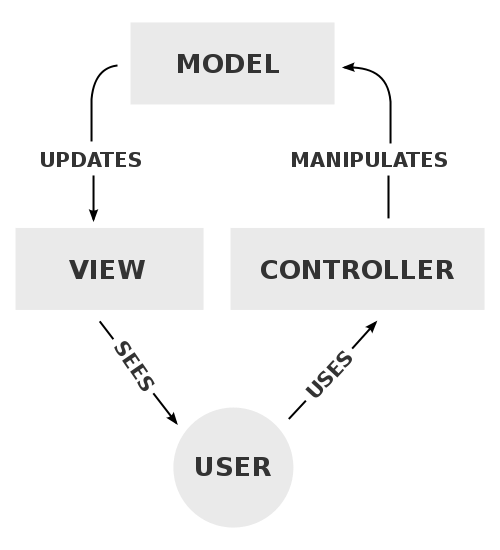
\includegraphics[width=0.5\columnwidth]{technical/MVC} 
\caption[MVC model]{Django appears to be an Model-View-Controller framework \cite{mvc_django}. It helped us to design properly Twinder.}
\label{fig:MVC_design} 
\end{figure}

The second framework that we used provides us with a simple design and structure to create dynamic slides. Many parameters are available, such as introducing a time for each slide or displaying the progression of the slides. However, we reduce Reveal to its minimum possible level in order to determine the influence to which the user is subject.

The two frameworks are available on GitHub: 
\begin{itemize}
  \item \textbf{Django}: \url{https://github.com/django/django}
  \item \textbf{Reveal}: \url{https://github.com/hakimel/reveal.js/}
\end{itemize}

The languages used have now been explained, allowing us to now focus on the general structure of the application.


\section{Structure}

\paragraph{}
We described previously the programming languages and the framework that we use to develop Twinder. In order to meet the expectations of the method, which is visualizing and giving their opinion on Tweets, we choose the duo Python / Javascript to build the apps. The framework Django gave us a structure for the entire architecture of the application and the database. \\
First we will explain to you the general structure of the application. Then, we will follow by describing the design of the database in detail.

\subsection{General structure}
\paragraph{}
The architecture of Twinder has evolved since the beginning of the project due to some constraints mainly coming from the API. Twitter limited the number of requests to the API, that is why, we chose the design that you can see above in figure \ref{fig:app_design}. \\

\begin{figure}[h] 
\centering 
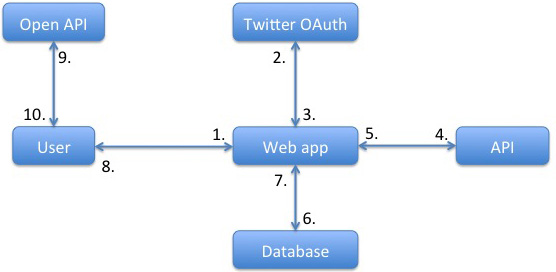
\includegraphics[width=1\columnwidth]{technical/AJAX} 
\caption[Connection with Twinder]{ The graph shows us the interactions with the API.
1. Connection to Twinder ;
2. Redirect to OAuth serveur ;
 3. Token is issued ;
  4. Request API + Token ;
  5. Answer ;
  6. Insert to db ;
  7. Retrieve from db ;
  8. Answer with tweets id ;
  9. Ajax call to Open API to get embed tweet ;
  10. Embed tweets.}
\label{fig:app_design} 
\end{figure}

Thanks to the diagram, you can see the essential steps required for the application to retrieve tweets from the API. In order to be more complete, we should add strides, necessary for the continuity of the process. Indeed, we registered Twinder to Twitter as an official app which allow us to get tokens for the authentication of our users. In figure \ref{fig:app_design}, you can see the run of the application which first starts with an Oauth delivered by a dedicate server, a token is issued. With this token, Twinder can request tweets to the API and then stores them in the database. As we explained previously, we now have 25 tweets times 10 friends in the database. After selecting 50 tweets to display, we send the list of ID's to the clients. Our method mentioned the fact that we should display embedded tweets in order to keep the context of the data. However, due to the API limits that we are going to explain after, we were not able to store the embed tweets directly in the database: we had to retrieve them from the client side. This step is represented by arrow 9 and 10, which show the AJAX call to the Twitter unauthenticated OEmbed endpoint. Indeed, as tweets are essentially public, it is possible to retrieve with their id, the embedded form without the constraint  of limited requests \cite{t_oembed1}.\\

\subsection{Important files}

\paragraph{}
Now that you understand the functioning of the application and the dependency linked to the API, we are going to describe the structure of the files dictated by Django. Figure \ref{fig:files} gives you the tree view of the application. We will briefly talk about three important files:  \textit{urls.py},  \textit{views.py} and  \textit{index.html}, the template. First, urls.py is a URL dispatcher which helps the developers keep a clean, elegant URL scheme. You can see above a sample of the code. We attribute to the address \textbf{\textit{base\_url/tweets}}, the function \textbf{\textit{index2}} which is in the file \textit{views.py}. 

 \lstinputlisting{code/py/url.py}

The next step is handled by views.py which contains all the backend functions. Functions are the logic of the application, if they are not internal, they are rendering templates with a context. This context is generated by the function itself and gives the content to the template index.html. As we saw in the previous chapter, balises enable the use of the backend data in HTML pages. After this overview of the Django structure, we are conducting a deep dive into the structure of the database. \\\\

\begin{figure}[h] 
\centering 
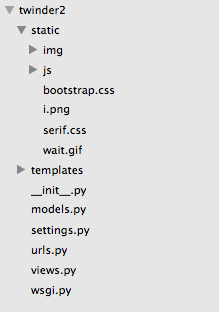
\includegraphics[width=0.4\columnwidth]{technical/files} 
\caption[MVC model]{Django comes with its own architecture. Statics files are the Javascript, CSS and the images. The templates are rendered by the data coming from views.py. Models.py generate the database structure and urls.py links the urls to function in views.py.}
\label{fig:files} 
\end{figure}

\subsection{Database}

\paragraph{}
We mentioned in the previous paragraph, three important files but we forgot a last one, models.py.
This file contains the model of our database and is defined by three classes as you can see with this code:

 \lstinputlisting{code/py/models.py}

The three classes: UnUser, UneSerie and LesTweets are composed by several fields and are linked together by Foreign Keys. \\
Now that you have a better understanding of the structure of the application and the database, we are going to scrutinise some interesting parts of the code.

\section{Parts of the code that is interesting}

\paragraph{}
In order to deep dive into the application, we are going to show you three central parts of the code which will give you a better understanding of Twinder. First of all, we describe the authentication process which allow the application to connect to the Twitter API. Next, we explain the javascript code which retrieves the opinion of the user for their tweet. Finally, we introduce to you the main function index which generates the vector of 50 tweets and render the html template.

\subsection{Authentication}

\paragraph{}
In order to retrieve tweets from a user thanks to the API, we need to first authenticate the candidate. As you can see above in figure \ref{fig:app_design}, the application is redirected to Twitter which will provide the login page. Line 4 of the code generates this redirection, and adds to this redirection the KEY and SECRET of the application which is registered on Twitter App \cite{t_dev_auth}. After that the user entered its credentials on Twitter, the application receives through a GET method, the token: get('oauth\_token') and the secret: get('oauth\_token\_secret') related to the user. \\
The final line returns an object which contains the credentials of the user and allow the program to query the API. As you probably noticed, we use the wrapper tweepy (ie. line 4 \& 6) in order to connect easily to the Twitter API with Python. We will discuss this more in detail in the section concerning the API. \\
After having provided the details of this authentication function, we will focus on the javascript function which retrieves and sends to the backend the opinion of the user for a given tweet.

 \lstinputlisting{code/py/oauth.py}

\subsection{Keyboard \& AJAX call}

\paragraph{}
The previous Python function which is in charge of the authentication is related to the backend. We will now jump to the front-end and explain the function which takes the decision of the user (like/dislike) and writes it on the database. This function written in Javascript can be split in two parts: the acquisition of the decision and the transmission of the decision.  \\
The acquisition of the information is handled by a library called KeyboardJS. Thanks to this library, the application is listening to the input coming from the two keys: F and L [Lines 25 and 26 of the code in annexe ]. When the user presses one of the two keys, it calls the function mark with different parameters depending on the choice of the user. "Mark" has to do the connection between the front-end and the back-end. Thanks to jQuery, the JavaScript library, it is possible to easily create an Ajax query. This query is composed by 3 attributes: the url, the type and the data. We are going to describe briefly these attributes:

\begin{itemize}
  \item \textbf{url}: thanks to the mapping function done by urls.py, the url is linked to the backend function which is ready to handle the data. 
  \item \textbf{type}: the POST method allows to transmit data to the backend without passing it through the url in plain text.
  \item \textbf{data}: it is the content transmited by the function to the backend function. In this case, we are sending a JSON with four components:  tweet\_id, friend\_id, txt\_lenght(number of characters in the tweet) and direction (left/right which is a mapping for like/dislike) 
\end{itemize}

Once the data is transmitted, if there is no error between the two sides, "mark" receives an answer from the backend. If data is false, it means that an error occurs in the backend. If this is not the case, the backend handles the JSON and inserts it into the database, creating a new object UneSerie. After having explained the communication between front-end and backend with the function mark, we will deep dive into the main function "index".

 \subsection{Index.html}
 
\paragraph{}
The index function is responsible of the rendering of the template. Before it calls the html page, we need to authenticate the user thanks to the authentication function line 8 that we describe previously. Then, we add the user to the database if it is not already in it. The next function called, is in charge of retrieving the tweets from the API and put them in the database. Some parameters were introduced in the function "retrieve\_tweets\_api" in order to change easily the number of friends or tweets to retrieve. Once the tweets are in the database, "retrieve\_from\_db" display the tweets to the user one-by-one.
For more informations, the code is available in annexe or Github \cite{tw_github} .

 \section{API}
 
 \paragraph{}
 In the previous chapters, we talk about the general structure of the application, the programming languages that we used and details some important parts of the code. However, we did not explain the API side which allows us to retrieve tweets. Firstly, we are going to talk about the wrapper that we used: Tweepy. Secondly, we will detail the request limitation of the API. Finally, we will point out the method that we found in order to foil this limits of the API. \\

\subsection{Wrapper}
 
\paragraph{} 
As we previously explained it, we use Python as backend language. In order to easily connect our application to Twitter API, it was necessary to use a wrapper library. As it is explains on Wikipedia: \textit{"a Wrapper libraries (or library wrappers) consist of a thin layer of code which translates a library's existing interface into a compatible interface. This is done for several reasons:
\begin{itemize}
  \item To refine a poorly designed or complicated interface.
  \item Allow code to work together which otherwise cannot (e.g. Incompatible data formats).
  \item Enable cross language and/or runtime interoperability."
\end{itemize}
}

Tweepy \cite{tweepy}, our wrapper library, allows us to easily connect Twinder to the API. Moreover, it is possible to get any object and use any method that the official Twitter API offers. The short sample of code gives you a good idea of how simple it is to retrieve information after having been authenticate.

 \lstinputlisting{code/py/tweepy.py}


 \subsection{Request limit}
 
 \paragraph{}
Once we connected our application to the Twitter API thanks to the wrapper Tweepy, we had to figure out how to deal with the request limit fixed by the company. Indeed, the twitter resources are not unlimited and computational power start to be consequent for platforms as big as Twitter. \\
A list is available on Twitter developer page \cite{t_rate_limit} and it gives the limit per service. Twinder is limited at several point has some limitations but the bottleneck is the Oembed request which is limited to 180 requests per user every 15min. As we load 250 tweets per person it was a critical issues to solve this problem. We finally found an interesting discussion \cite{t_oembed2}:

\textit{You should find that you're able to fetch as many embed codes as you need from the unauthenticated OEmbed endpoint. Rate limits are not applied to this endpoint in the same way as for API v1.1.}

We bypassed the limitation by using a public OEmbed endpoint which is reach by a GET ajax request:

 \lstinputlisting{code/stream.js}


After having explained the limit issues coming from the API and our solution. We will talk about the versioning tools that we employ: Git and Heroku.

 \section{Deployment}
 
  \paragraph{}
 In order to manage this project, we use two services essentials in web programmation. On the one side, Github is a Git repository web-based hosting service useful to track the bug in our case. On the other side, Heroku is a cloud platform as a service and allows us to deploy directly from Github our project.
You can find the code open source of Twinder on Github \cite{tw_github} and the application on Heroku \cite{tw_heroku}.




